\documentclass[conference]{IEEEtran}


\usepackage[latin1]{inputenc}
\usepackage{hyperref}
\usepackage{amsmath}
\usepackage{amssymb}
\usepackage{color}
\usepackage{amsfonts}
\usepackage{mathtools}
\usepackage{algorithm2e}
\usepackage{graphicx}
\usepackage{fixme}
\usepackage{tikz}
\usepackage{pgfplots}
\usepackage{xcolor}
\usepackage[justification=centering]{caption}
\usepackage{flexisym}
\newcommand\TODO[1]{\textcolor{red}{#1}}
\pgfplotsset{compat=1.9}
\usetikzlibrary{arrows}
\usetikzlibrary{positioning,calc}
\usetikzlibrary{decorations.pathreplacing}
\usetikzlibrary{decorations.markings}
\usetikzlibrary{fit}
\usetikzlibrary{shapes.callouts}
\usetikzlibrary{shapes.geometric}
\usetikzlibrary{matrix}
\usetikzlibrary{spy}

\usepackage{expl3}
\ExplSyntaxOn
\newcommand\latinabbrev[1]{
  \peek_meaning:NTF . {% Same as \@ifnextchar
    #1\@}%
  { \peek_catcode:NTF a {% Check whether next char has same catcode as \'a, i.e., is a letter
      #1.\@ }%
    {#1.\@}}}
\ExplSyntaxOff


\newcommand{\todo}[1]{\textcolor{red}{TODO: #1}\PackageWarning{TODO:}{#1!}}
\def\ie{\latinabbrev{i.e}}


\newcommand{\norm}[1]{\left\lVert #1 \right\rVert}
\def\doubleunderline#1{\underline{\underline{#1}}}
\renewcommand{\vec}[1]{\boldsymbol{#1}}
\newcommand{\p}[1]{\left(#1\right)}
\newcommand{\f}[2]{\frac{#1}{#2}}
\newcommand{\de}[1]{\begin{vmatrix}#1\end{vmatrix}}
\newcommand{\m}[1]{\begin{pmatrix}#1\end{pmatrix}}
\newcommand{\ub}[1]{\underbrace{#1}}
\newcommand{\ubt}[2]{$\underbrace{\mbox{#1}}_{\mbox{#2}}$}
\newcommand{\comb}[2]{{#1 \choose #2}}
\newcommand{\Z}{{\mathbb{Z}}}
\newcommand{\Q}{{\mathbb{Q}}}
\newcommand{\R}{{\mathbb{R}}}
\newcommand{\C}{{\mathbb{C}}}
\newcommand{\N}{{\mathbb{N}}}
\newcommand{\wC}{{\textit{C}}}
\newcommand{\n}{\vskip 6pt \noindent}
\newcommand{\e}{\epsilon}
\newcommand{\notdv}{\thinspace \not | \thickspace}
\newcommand{\union}{\cup}
\newcommand{\inter}{\cap}
\newcommand{\into}{\rightarrow}
\newcommand{\nset}[1]{#1_1,\ldots,#1_n}
\newcommand{\setk}[2]{#1_1,\ldots,#1_#2}
\newcommand{\bnset}[1]{\{#1_1,\ldots,#1_n\}}
\newcommand{\bset}[2]{\{#1_1,\ldots,#1_#2\}}
\newcommand{\ton}[1]{#1=1,\ldots,n}
\newcommand{\tok}[2]{#1=1,\ldots,#2}
\newcommand{\disc}{\operatorname{disc}}
\newcommand{\spn}{\operatorname{Span}}
\newcommand{\rank}{\operatorname{rank}}
\newcommand{\proj}{\operatorname{proj}}
\newcommand{\prp}{\operatorname{perp}}
\newcommand{\ux}{\underline{x}}
\newcommand{\ua}{\underline{a}}
\newcommand{\uu}{\underline{u}}
\newcommand{\pfx}{\frac{\partial f}{\partial x}}
\newcommand{\pfy}{\frac{\partial f}{\partial y}}
\newcommand{\px}{\frac{\partial}{\partial x}}
\newcommand{\pxn}[1]{\frac{\partial f}{\partial x_{#1}}}
\newcommand{\py}{\frac{\partial}{\partial y}}
\newcommand{\jacu}{\frac{\partial(u,v)}{\partial(x,y)}}
\newcommand{\jacx}{\frac{\partial(x,y)}{\partial(u,v)}}
\newcommand{\vzero}{\vec{0}}
\newcommand{\va}{\vec{a}}
\newcommand{\vb}{\vec{b}}
\newcommand{\vc}{\vec{c}}
\newcommand{\vd}{\vec{d}}
\newcommand{\ve}{\vec{e}}
\newcommand{\vh}{\vec{h}}
\newcommand{\vn}{\vec{n}}
\newcommand{\vs}{\vec{s}}
\newcommand{\vu}{\vec{u}}
\newcommand{\vv}{{\vec{v}}}
\newcommand{\vw}{\vec{w}}
\newcommand{\vx}{\vec{x}}
\newcommand{\vy}{\vec{y}}
\newcommand{\vz}{\vec{z}}
\newcommand*{\everymodeprime}{\ensuremath{\prime}}
\begin{document}

\title{Neural Machine Translation}
\vspace{-1.5cm}
\author{\IEEEauthorblockN{Seminar Report-NLP}
\IEEEauthorblockN{Arul, Ehsan}
\IEEEauthorblockA{Rheinische Friedrich-Wilhelms-Universit\"at Bonn}
\IEEEauthorblockA{\today}
}

\maketitle


\begin{abstract}
Abstract

\end{abstract}


\section{Introduction}


\section{Deep Learning - An Introduction}

In the recent  years, Deep learning has been making a big impact in various fields of computer science. This impact is profound in the perceptual learning task in the fields like computer vision, natural language processing, etc, \cite{lecun2015deep}. Though the idea of training a multi layered neural network to perform function approximation is known to the research community for at least a couple of decades\cite{schmidhuber2015deep}, due to the nature of training problem requiring large computational resources, the multi layered neural network remained less practical. With the advent of general purpose graphical processing units(GPGPUs) and the availability of training data, the neural networks are now a practical solution for many perceptual tasks. One of the early success of deep learning was in the field of image classification. In the annual ImageNet classification challenge \cite{deng2009imagenet}, AlexNet \cite{krizhevsky2012imagenet} showed a remarkable improvement in the state-of-the-art accuracy. Within a few years, more sophisticated architectures like Google Inception Network \cite{szegedy2016rethinking}, Deep Residual Network \cite{he2016deep}, etc., has improved the accuracy to be comparable with a human in that task. The generality of the neural network made it easily possible to be used for a wide variety of tasks. With more people working on deep learning and the ideas arising in solving on the problems being easily transferable, the deep learning is the state-of-the-art for many learning tasks. In the following section, we will briefly summarize the basics of deep learning.


The basic building block of a Multilayer network, or in more technical term Multilayer  perceptron(MLP) is a perceptron. The preceptron \ref{fig:ann} closely resembles a neuron in a human brain \ref{fig:neuron}. A preceptron takes a set of input values, computes a weighted sum of the inputs, and outputs a scalar value of a after applying an activation function (mostly non-linear). The weights for computing the weighted sum and the threshold in the activation function are initially set to random values and are learned from the training data. 
Mathematically, a perceptron with the weight matrix $A$ and the threshold $T$ for an step activation function, for the input vector $x$, outputs the following,


\[
    f(x)= 
\begin{cases}
    1,& \text{if }  A x > c \\
    0,              & \text{otherwise}
\end{cases}
\]

A layer has many number of neurons and many layers are stacked one on top of the other to form a MLP. An MLP with very many layers is called as Deep Neural Network(DNN). In the following section we will discuss the properties of DNNs and how they are useful in the context of supervised machine learning.


\begin{figure}
    \includegraphics[width=.99\linewidth]{img/bioneuron.jpg}  
    \caption{A biological neuron.}
    \label{fig:neuron}
\end{figure}

\begin{figure}
    \includegraphics[width=.99\linewidth]{img/artificial.jpg}  
    \caption{ An artificial neuron (perceptron)}
    \label{fig:ann}
\end{figure}


\begin{figure}
    \includegraphics[width=.99\linewidth]{img/mlp.png}  
    \caption{Layered representation in an MLP}
    \label{fig:mlp}
\end{figure}


\subsection{Supervised learning}
Supervised learning is the problem of predicting an new output $y\everymodeprime$  for a new input $x\everymodeprime$, and set of training data that provides a set of input and output $\{x \mapsto y\}$. Most of the supervised learning problems can be formulated as either a classification or regression problem. Classification is the problem of predicting the label for a given  $x\everymodeprime$ among a set of given labels $\{Y\}$ while regression of predicting a continuous  valued output for a given input. The usual way of doing supervised learning is to extract features from the given data and train a model to perform classification or regression. 


$$x \xrightarrow[\text{Feature extraction}]{ \mathbb{D}(x) } x\everymodeprime _{intermediate} \xrightarrow[\text{classifer/regressor}]{\mathbb{F}(x\everymodeprime | \theta)}   y$$

The power of the DNNs lie in the fact that the models learns the features directly from the given training data and avoids hand engineered features. 
$$ x \xrightarrow[ \text{hierachical}] { \mathbb{M}(x | \Theta) } y$$
\bibliographystyle{plain}

The DNNs with neurons in one layers being connected to all the neurons in the next layer are called Feed Forward Networks. The feed forward networks are harder to train since they have lots of parameters. To make a the DNNs learn useful representation for performing supervised learning, we need special types of connections between the neurons. Two of the most commonly used DNN architectures are Convolutional Neural Networks(CNN) and Recurrent Neural Networks(RNN). In the following section we will discuss these architectures in detail.


\subsubsection{CNN}
todo

The Convolutional NN are shown in \ref{fig:cnn}

\begin{figure}
    \includegraphics[width=.99\linewidth]{img/cnn.png}  
    \caption{CNN}
    \label{fig:cnn}
\end{figure}



\begin{figure}
    \includegraphics[width=.99\linewidth]{img/rnn.png}  
    \caption{Recurrent connections in a RNN}
    \label{fig:rnn}
\end{figure}

\begin{figure}
    \includegraphics[width=.99\linewidth]{img/lstm_forget.png}  
    \caption{Forget gate in LSTM} 
    \label{fig:lstm_forget}
\end{figure}

\begin{figure}
    \includegraphics[width=.99\linewidth]{img/lstm_add.png}  
    \caption{Add gate computing parts to be to modified in LSTM} 
    \label{fig:lstm_add}
\end{figure}

\begin{figure}
    \includegraphics[width=.99\linewidth]{img/lstm_add1.png}  
    \caption{Add gate computing data to be added to cell state in LSTM} 
    \label{fig:lstm_add1}
\end{figure}


\begin{figure}
    \includegraphics[width=.99\linewidth]{img/lstm_output.png}  
    \caption{Add gate computing output in LSTM} 
    \label{fig:lstm_output}
\end{figure}

\begin{figure}
    \includegraphics[width=.99\linewidth]{img/enc_dec.png}  
    \caption{Simple Encoder-Decoder architecture for machine translation} 
    \label{fig:enc_dec}
\end{figure}


\subsubsection{RNN}
The neurons in the RNNs have recurrent self connections. \ie The output of the neurons are connected back to the inputs. Thus the output at time step $t_1$ is computed with taking output at time step $t_0$ as input. The recurrent connections are shown Fig.\ref{fig:rnn} This enables the RNNs to have an internal memory. RNNs are trained with the a modified version of back propagation called \textbf{Back Propagation Through Time(BPTT)}  \cite{werbos1990backpropagation}.

RNNs in general are harder to train and this is particularity evident when the BPTT is done over a larger number of time steps. This is because the gradients simply converges to zero after a few time steps. This problem known as \textbf{vanishing gradients problem} is a well studied phenomenon \cite{bengio1994learning}.  

To alleviate the vanishing gradients problem, a special architecture called \textbf{Long Short Term Memory(LSTM)} \cite{hochreiter1997long} is used. An LSTM cell is shown in \label{fig:lstm}.

LSTM cells has separate internal memory vector and has three gates--forget gate, add gate, and output gate. To understand the Mathematical intuition behind these gates, let us consider a LSTM cell in a hidden state $h$ and internal cell memory vector $c_{t-1}$. At time $t$, the cell takes input $x_t$, previous output $h_{t-1}$ and update the cell memory to $c_{t}$, produces the output $h_{t}$. The forget computes a vector size $c$ between 0 and 1. This vector determines who information should be preserved and what should be forgotten based on the current input $x_t$ as shown in \ref{fig:lstm_forget}. This vector is later multiplied with the cell memory. If the vector is all zeros, multiplying makes all cell state to forget everything while all ones preserve everything. Then the add gate computes which parts in the cell states to be updates as shown in  \ref{fig:lstm_add} and the new data to be updated as shown in \ref{fig:lstm_add1}. Finally the output gate generates the output $h_t$ and does not modify the cell state as shown in \ref{fig:lstm_output}.




\subsection{Related work}
PBMT explanation. \cite{koehn2003statistical} 

\subsection{Neural Machine Translation}
Though usage of neural networks did not yield promising results in the early years, the recurrent neural networks started to achieve performance comparable to PBMT as in \cite{kalchbrenner2013recurrent} and \cite{hermann2013multilingual}. Most of the early architectures were simple encoder-decoder architectures. An simple working of encoder-decoder architecture for machine translation is shown in Fig.\ref{fig:enc_dec}. The architecture has an encoder that takes a sentence in source language and encodes it into a vector $S$ of fixed length. The decoder takes the embedding $S$ as input and generates the sentence in the target language. Some of the major drawbacks with the simple architecture is that
\begin{enumerate}
 \item The encoder has to encode all the information in the source sentence into fixed size embedding $S$. 
 \item The decoder never sees the actual input sentence and has to rely completely on $S$ for generating target sentence. 
 \item Having fixed size embedding vector makes the architecture less flexible. Smaller size means less information where as using larger vector means for smaller sentences we need zero padding and more computation time.
\end{enumerate}


\begin{figure}
    \includegraphics[width=.99\linewidth]{img/context.png}  
    \caption{Context for machine translation} 
    \label{fig:context}
\end{figure}

\subsubsection{Jointly learning to align and translate}
The paper \cite{bahdanau2014neural} address this issue of having a fixed size embedding by introducing the idea of context \ref{fig:context}. The main proposal was to use
\begin{enumerate}
 \item Encoder outputs a hidden representation for each word in the source sentence $F_s$.
 \item One context vector $C$ in the size of the input sentence that has values between 0 and 1.
 \item Each element of the embedding $F_s$ is multiplied with one element in $C$.
\end{enumerate}
The whole embedding is made available to the decoder and $C$ describes which part of the embedding should be focused to generate the current word based on the previous word.

Encoder RNN, at each input step t, generates hidden state, $h_t = f(x_t, h_{t-1})$.

Unlike in the previous models where only the last hidden state is made available to the decoder, this paper provided all the hidden state and also a context vector that has a weight for each of the hidden vector. The context vector helps the decoder to focus on a part of the sentence. $c = q(\{h_1,\cdots,h_{T_x}\})$. 

The decoder is trained to predict the next work $y_t$ given the context vector $c$ and all previously predicted words $\{ y_1, \cdots, y_{t-1}\}$
 $$ p(y) = \prod^{T}_{t=1} p(y_t | \{ y_1, \cdots, y_{t-1}\} ,c ) $$
 With RNN, each conditional probability is modeled as,
 $$ p(y_t | \{ y_1, \cdots, y_{t-1}\}, c) = g(y_{t-1}, s_t, c) $$ where $s_t$ is the hidden state of the RNN.
 The context vector for a input sentence $i$, is computed as a weighted sum of hidden states of the encoder (also known as \textbf{annotations})
  $$ c_i = \sum_{j=1}^{T_{x}} \alpha_{ij} h_j$$
  $$ \alpha_{ij} = \frac{ exp(e_{ij})}{ \sum_{k=1}^{T_x} exp (e_{ik})}$$

where,
$$ e_{ij} = a(s_{i-1}, h_j)  $$ is the alignment model that scores how well the inputs around the $j$ and the output at the position $i$ match.

A feedforward neural network is used as the alignment model and is \textbf{jointly trained} with all the NMT system as a whole.

 \begin{figure}
    \includegraphics[height=8cm]{img/contextres.png}  
    \caption{Visualization of the context in action}
    \label{fig:contextvis}
  \end{figure}
  

The functionality of the context vector is visualized in the Fig. \ref{fig:contextvis}. For example, the French language has the words  \textquotedblleft European Economic Area\textquotedblright exists in the reverse order as \textquotedblleft zone \'{e}conomique europ\'{e}enne\textquotedblright. The context learns to focus on the correct order for the decoder. 



\begin{figure}
    \includegraphics[width=0.9\linewidth]{img/birnn.png}  
    \caption{Bi-directional Encoder}
    \label{fig:birnn}
\end{figure}

This paper also made use of the bi-directional LSTM in the layers of the Encoder. Just like an LSTM that has an internal memory to comprehend the past states, the LSTM also comprehends the words that comes next in the sentence. It has two internal state---one for past states and one for the future state. A bi-directional LSTM is shown in \ref{fig:birnn}.


The whole model is trained with standard maximum-likelihood error minimization $\mathbb{O}_{ML}(\Theta) = \sum_{i=1}^N log P_\Theta(Y^{*(i)} | X^{(i)}) $ with stochastic gradient descent(SGD) on a mini-batch of 80 sentences. For the first time, the BLEU score was comparable to phrase based machine translation system. But the fact that there are no individual pieces in the model was a great benefit and the research community started to consider neural systems as an viable alternative phrase based machine translation system.


\subsubsection{Sequence to Sequence models.}
With in an year, more deep and powerful models were computationally possible. Taking the availability of the computational power to advantage a new framework for learning sequence to sequence mapping were proposed. A sequence to sequence model formulated as 
$$ p(y_1, \cdots, y_T| x_1, \cdots, x_T) = \prod_{t=1}^{T} p(y_t| v, y_1, \cdots, y_{t-1})$$
where $v$ is the internal memory of the RNNs. With more powerful RNNs, this model can be used to learn a variety of tasks like speech recognition, handwritten digits recognition, machine translation, etc as shown in the paper \cite{sutskever2014sequence}


 \begin{figure}
 \centering
      \includegraphics[width=.49\linewidth]{img/seq2seq.pdf} 
	\caption{ Seq2Seq model}
	\label{fig:seq}
\end{figure}


 \begin{figure}
  \centering
      \includegraphics[width=.49\linewidth]{img/seq2seq_deep.pdf} 
	\caption{A more powerfuls Seq2Seq model}
	\label{fig:seqdeep}
\end{figure}


 \begin{figure}
  \centering
      \includegraphics[width=.9\linewidth]{img/wordvec.png} 
	\caption{Two-dimensional PCA projection of the 1000-dimensional word embedding.}
	\label{fig:wordvec}
\end{figure}
A simple sequence to sequence model is shown in  Fig.\label{fig:seqdeep}. Just by making the model more deeper, without any special treatment for machine translation, the paper achieved state-of-the art results. The model as trained on WMT English to French dataset with 12M sentences consisting of 348M French words and 304M English words using 160,000 of the most frequent words for the source language and 80,000 of the most frequent words for the target language. Every out-of-vocabulary word was replaced with a special \textbf{UNK} token. The network has 4 LSTM layers with 1000 LSTM cells in each layer. The paper used 1000 dimensional word embedding to represent the words as vector following the word2vec paper \cite{mikolov2013distributed}. word2vec formulated the problem of learning word embedding as an energy maximization problem using a simple neural network with just one hidden layer. The energy maximized is called Negative sampling. The resulting vector embedding is empirically shown to have arithmetic properties. \ie  $\,$France - Paris + Germany is roughly equal to Berlin as shown in Fig.\ref{fig:wordvec}. The paper an impressive BLEU score of 33.3 even without doing anything specific for machine translation.

\bibliography{literature}
\end{document}



